\begin{enumerate}[label=\thesubsection.\arabic*,ref=\thesubsection.\theenumi]
% =========================================================
%\section*{1. Geometric Progression of Frequencies}
	\iffalse
\item Geometric Progression of Frequencies

If each successive term is $r$ times the previous term, then after
$k$ steps from a reference term $f_0$,

\begin{align}
\frac{f_k}{f_0}=r^{k}. \label{GP}
\end{align}


%\end{enumerate}
% =========================================================
\item Self-Similar (Fractal) Curve Length

If, at every iteration, each segment is replaced by $m$ segments each
of length $\dfrac{1}{p}$ of the original segment, the length scales as

\begin{align}
L_1&=L_0\left(\frac{m}{p}\right),\\
L_n&=L_0\left(\frac{m}{p}\right)^{n}. \label{iteration}
\end{align}
\fi
% =========================================================
\item (Rolle's Theorem)
	\label{prop:rolle}
If $f$ is continuous on $[a,b]$, differentiable on $(a,b)$, and
$f(a)=f(b)$, then
\begin{align}
\exists\, c\in(a,b)\ \text{such that}\ f'(c)=0.
	\label{eq:EE26BTECH11221-rolle}
\end{align}
%Contrapositive form: if $f'(x)\neq 0$ for all $x$, then
%$f(a)\neq f(b)$ for $a\neq b$.
% =========================================================
\item (Closed-Loop Transfer Function)
For unity negative feedback with forward transfer function $G(s)$,
  in \figref{fig:EE26BTECH11221-unity-feedback},
the transfer function is given by 
\begin{align}
\frac{Y(s)}{X(s)}=\frac{G(s)}{1+G(s)}. 
\label{eq:EE26BTECH11221-neg}
\end{align}
	\begin{figure}[H]
  \centering
  \resizebox{0.75\columnwidth}{!}{%
	      \begin{tikzpicture}[
        >=stealth,
        block/.style={
            draw,
            rectangle,
            minimum width=4cm,
            minimum height=1.5cm
        },
        sum/.style={
            draw,
            circle,
            minimum size=0.9cm
        }
    ]

    % Summing junction
    \node[sum] (sum) {};

    % Plus and minus signs
    \node at ($(sum.center)+(-0.2,0.0)$) [font=\tiny] {$+$};
    \node at ($(sum.center)+(0.0,-0.2)$) [font=\tiny] {$-$};

    % Input arrow with label X(s)
    \draw[->] ($(sum.west)+(-1.2,0)$) node[left] {$X(s)$} -- (sum.west);

    % Transfer function block
    \node[block, right=0.8cm of sum] (G)
    {
        $G(s)$
        %$G(s)=\dfrac{25}{s(s+5)}$
    };

    % Forward path
    \draw[->] (sum.east) -- (G.west);

    % Output arrow with label Y(s)
    \draw[->] (G.east) -- ++(1.2,0) node[right] {$Y(s)$};

    % Feedback line
    \draw (G.east) -- ++(0.5,0)
        |- ($(sum.south)+(0,-1.3)$)
        -- (sum.south);

    \end{tikzpicture}%


  }
  \caption{Unity feedback}
  \label{fig:EE26BTECH11221-unity-feedback}
\end{figure}
%
% =========================================================
% QUESTION 10
% =========================================================
\item (Nyquist Sampling Theorem \label{sampling}) A time domain signal is given by
\begin{align}
x(t) = 20\sin(100\pi t) + 36\sin(150\pi t) - 2\sin(300\pi t),
\end{align}
where time $t$ is in seconds. Among the following options, what is the frequency (in $\text{Hz}$) at which $x(t)$ should be sampled for accurate signal reconstruction?
\hfill  (BM 2025)
% =========================================================
% OPTIONS
% =========================================================
\begin{multicols}{4}
\begin{enumerate}
\setlength{\itemsep}{0pt}
    \item $500$
    \item $150$
    \item $200$
    \item $250$
\end{enumerate}
\end{multicols}
% =========================================================
% SOLUTION
% =========================================================
\solution
The frequencies of the three sinusoidal components are
\begin{align}
f_1 &= \frac{100\pi}{2\pi} = 50\text{ Hz}
f_2 &= \frac{150\pi}{2\pi} = 75\text{ Hz}
f_3 &= \frac{300\pi}{2\pi} = 150\text{ Hz}
\end{align}
According to the Nyquist theorem, the sampling rate  is
\begin{align}
f_s \ge 2 \times f_3  = 300\text{ Hz}.
    \label{eq:EE26BTECH11221-sampling}
\end{align}
Among the given options, the only frequency greater than or equal to $300\text{ Hz}$ that guarantees accurate signal reconstruction is $500\text{ Hz}$.
The following code generates
    \figref{fig:EE26BTECH11221-sampling}.
\begin{lstlisting}
Codes/bm10.py
\end{lstlisting}
\begin{figure}[H]
    \centering
    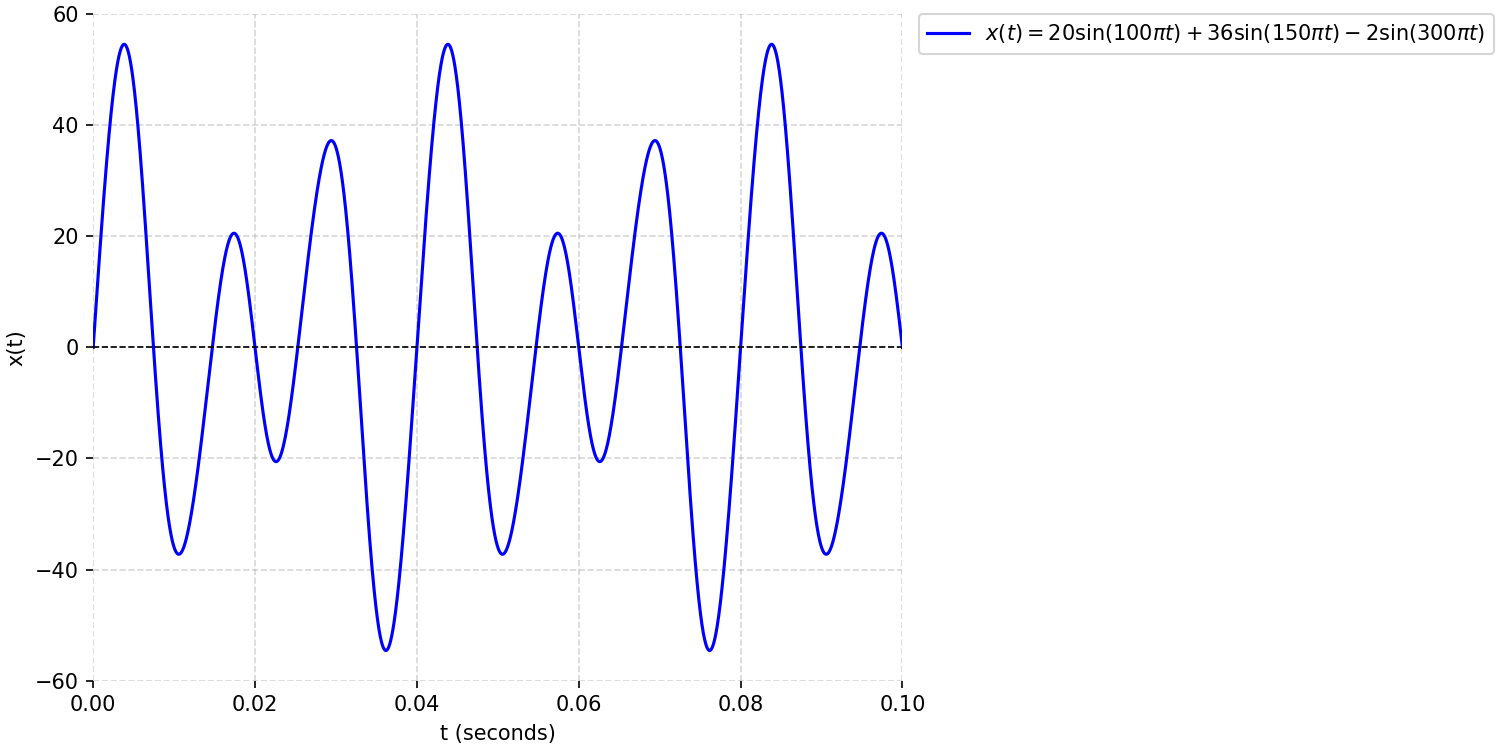
\includegraphics[width=1\textwidth]{figs/bm10.png}
    \caption{Plot of x(t) vs time}
    \label{fig:EE26BTECH11221-sampling}
\end{figure}
% =========================================================
\item Average Power in an AC Circuit
\begin{align}
P_{\text{avg}}=V_{\text{rms}}I_{\text{rms}}\cos\theta, \label{power}
\end{align}

where

\begin{align}
V_{\text{rms}}&=\frac{V_m}{\sqrt2}\\
I_{\text{rms}}&=\frac{I_m}{\sqrt2}\\
\theta&=\phi_v-\phi_i.
\end{align}

% =========================================================
\item 
	\begin{align}
		E\brak{X^n} = \frac{d}{dt^n}\sbrak{M_X\brak{e^{-t}}}_{t=0} 
\label{eq:EE26BTECH11221-moment-n-mgf_xz}
\end{align}
\solution
From 
\eqref{eq:EE26BTECH11213-mgf-def},
%\eqref{eq:EE26BTECH11221-dice_xz},
	\begin{align}
		\frac{d}{dt^n}\cbrak{M_X\brak{e^{-t}}} &= 
		\sum_{k=-\infty}^{\infty}k^np_X\brak{k} e^{kt} 
\end{align}
yielding
\eqref{eq:EE26BTECH11221-moment-n-mgf_xz}.
	\item For the Binomail distribution $X \sim \bnm{n}{p}$,
		\begin{align}
			\label{moment-mean-var}
			\mu = np, \sigma^2 = npq
		\end{align}
		\solution 
From 
\eqref{eq:EE26BTECH11221-moment-n-mgf_xz},
%and 
%\eqref{eq:mgf-binom},
\begin{align}
	E\brak{X}&=\frac{d}{dt}\cbrak{\brak{q+pe^{t}}^n}_{t=0} 
	\\
		 &= \lim_{t=0}np\brak{q+pe^{t}}^{n-1}=np
\label{eq:EE26BTECH11221-binom-mean}
\end{align}
and
\begin{align}
	M_X^{\prime}\brak{t} &= n\brak{q + p e^t}^{n-1}pe^t
	\\
M_X^{\prime \prime}\brak{t}
&= n\brak{n-1}\brak{1 - p + p e^t}^{n-2}\brak{p e^t}^2 \\
&\quad + n\brak{1 - p + p e^t}^{n-1}\brak{p e^t}
\end{align}
Therefore
\begin{align}
	E\brak{X^2}
&= n\brak{n-1}p^2 + np
\\
	\implies \text{var}\brak{X} &= 
	E\brak{X^2}
-E\brak{X}^2=
npq
\label{eq:EE26BTECH11221-binom-variance}
\end{align}
%\end{enumerate}
%
\item Mean and Variance of a Binomial Distribution
For $X\sim B(N,p)$,
\begin{align}
E(X)&=Np\\
\operatorname{Var}(X)&=Np(1-p). \label{variance}
\end{align}

% =========================================================
% QUESTION 14
% =========================================================
\item In the circuit shown  in 
  \figref{fig:EE26BTECH11221-ckt}
	below, $V_{\text{in}} = 10\cos(1000t)\text{ volts}$. The magnitude of the input impedance of the circuit is 
\underline{\hspace{2cm}} $\text{k}\Omega$. 
\hfill  (BM 2025)
	\begin{figure}[H]
  \centering
  \resizebox{0.75\columnwidth}{!}{%
	  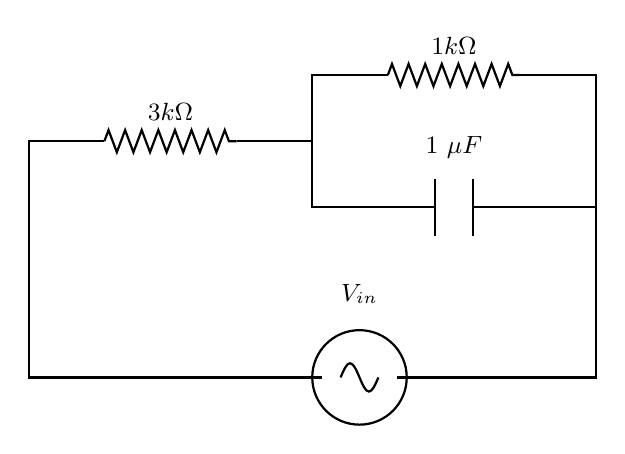
\begin{tikzpicture}[scale=1.2, every node/.style={font=\small}]

  % Top left wire & 3 k\Omega resistor
  \draw[thick] (0,-1) -- (0,1.5) -- (0.8,1.5);
  \draw[thick, decorate, decoration={zigzag, segment length=6pt, amplitude=4pt}] (0.8,1.5) -- (2.2,1.5);
  \node[above=4pt] at (1.5,1.5) {$3\text{ k}\Omega$};
  \draw[thick] (2.2,1.5) -- (3,1.5);
  
  % Parallel top branch: 1 k\Omega resistor
  \draw[thick] (3,1.5) -- (3,2.2) -- (3.8,2.2);
  \draw[thick, decorate, decoration={zigzag, segment length=6pt, amplitude=4pt}] (3.8,2.2) -- (5.2,2.2);
  \node[above=4pt] at (4.5,2.2) {$1\text{ k}\Omega$};
  \draw[thick] (5.2,2.2) -- (6,2.2) -- (6,1.5);
  
  % Parallel bottom branch: 1 \mu F capacitor
  \draw[thick] (3,1.5) -- (3,0.8) -- (4.3,0.8);
  \draw[thick] (4.3,0.5) -- (4.3,1.1);
  \draw[thick] (4.7,0.5) -- (4.7,1.1);
  \node[above=4pt] at (4.5,1.1) {$1\ \mu\text{F}$};
  \draw[thick] (4.7,0.8) -- (6,0.8);
  
  % Outer connections & AC Source
  \draw[thick] (6,1.5) -- (6,-1) -- (3.9,-1);
  \draw[thick] (0,0) -- (0,-1) -- (3.1,-1);
  \draw[thick] (3.5,-1) circle (0.5);
  \draw[thick] (3.3,-1) sin (3.4,-0.85) cos (3.5,-1) sin (3.6,-1.15) cos (3.7,-1);
  \node[above=6pt] at (3.5,-0.5) {$V_{\text{in}}$};
\end{tikzpicture}


  }
  \caption{Steady state analysis.}
  \label{fig:EE26BTECH11221-ckt}
\end{figure}
% =========================================================
% OPTIONS
% =========================================================
\begin{multicols}{4}
\begin{enumerate}
\setlength{\itemsep}{0pt}
    \item $5.0$
    \item $3.5$
    \item $6.0$
    \item $4.5$
\end{enumerate}
\end{multicols}
% =========================================================
% SOLUTION
% =========================================================
\solution
The input impedance can be expressed as
\begin{align}
	R_1 + R_2 \parallel \frac{1}{\j \omega C}
	&=
	R_1+\frac{R_2 \brak{\frac{1}{\j\omega C}}}{R_2 + \frac{1}{\j\omega C}}\\
	\\
	&=
	R_1+\frac{R_2}{\j\omega CR_2 + 1}
    \label{eq:EE26BTECH11221-impedance}.
=
3.5 - j0.5
\end{align}
upon substituting the following values in
    \eqref{eq:EE26BTECH11221-impedance} and simplifying.
\begin{align}
R_1 = 3k \ohm,
\quad R_2 = 1\text{k}\ohm, \quad C = 1\,\mu\text{F}, \quad \omega = 1000\text{ rad/s}.
\end{align}
The following code plots 
    \figref{fig:eq:EE26BTECH11221-impedance}.
\begin{lstlisting}
Codes/bm14.py
\end{lstlisting}
\begin{figure}[H]
    \centering
    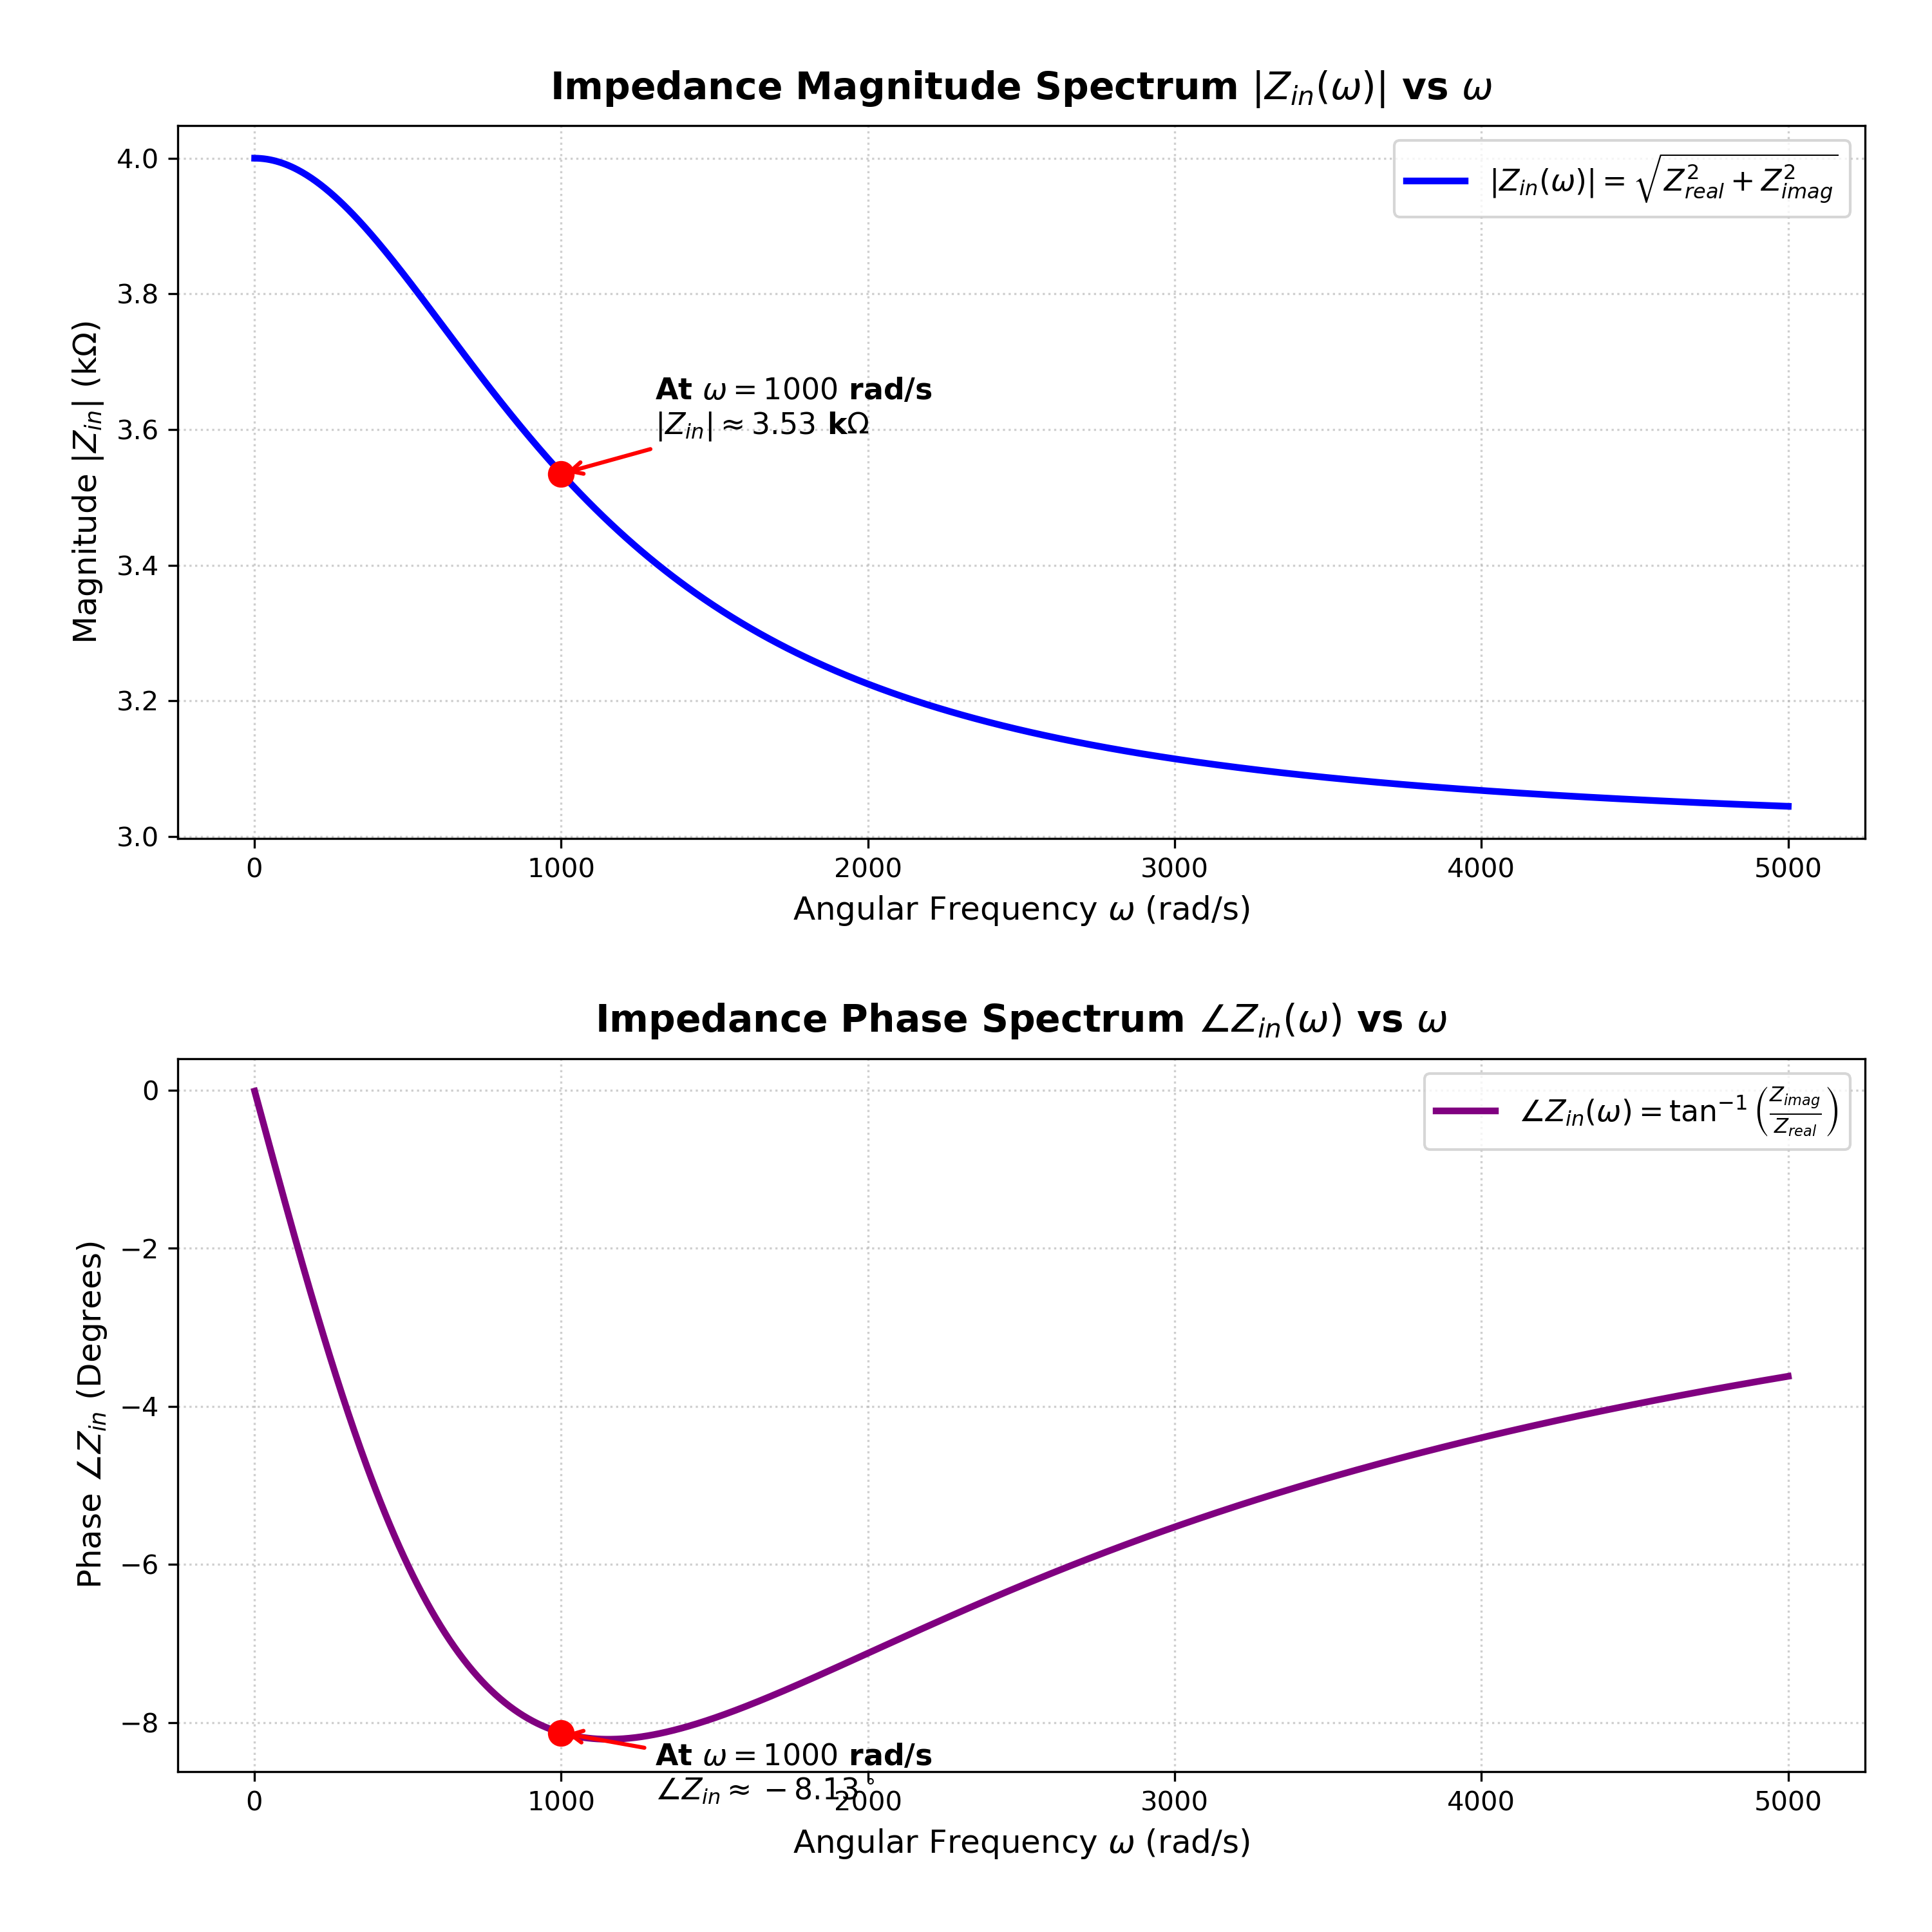
\includegraphics[width=1\textwidth]{figs/bm14.png}
    \caption{Magnitude and Phase.}
    \label{fig:eq:EE26BTECH11221-impedance}
\end{figure}
% =========================================================
% QUESTION 16
% =========================================================
\item Two systems $U$ and $V$ are defined as shown below
	in
  \figref{fig:EE26BTECH11221-lin-cause}.
	Which of the following statement(s) is/are CORRECT?
\hfill  (BM 2025)
	\begin{figure}[H]
  \centering
  \resizebox{0.75\columnwidth}{!}{%
	  
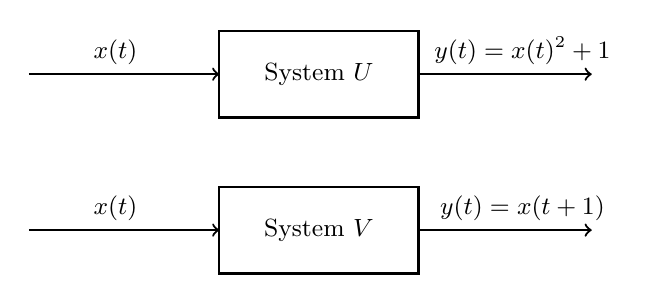
\begin{tikzpicture}[scale=1.1, every node/.style={font=\small}]

    % System U block and arrows
    \draw[thick] (0,1.8) -- (1.5,1.8);
    \draw[thick, ->] (1.5,1.8) -- (2.2,1.8);
    \node[above] at (1.0,1.8) {$x(t)$};

    \draw[thick] (2.2,1.3) rectangle (4.5,2.3);
    \node at (3.35,1.8) {System $U$};

    \draw[thick, ->] (4.5,1.8) -- (6.5,1.8);
    \node[above] at (5.7,1.8) {$y(t) = x(t)^2 + 1$};

    % System V block and arrows
    \draw[thick] (0,0) -- (1.5,0);
    \draw[thick, ->] (1.5,0) -- (2.2,0);
    \node[above] at (1.0,0) {$x(t)$};

    \draw[thick] (2.2,-0.5) rectangle (4.5,0.5);
    \node at (3.35,0) {System $V$};

    \draw[thick, ->] (4.5,0) -- (6.5,0);
    \node[above] at (5.7,0) {$y(t) = x(t + 1)$};

\end{tikzpicture}

  }
  \caption{Linearity and Causality}
  \label{fig:EE26BTECH11221-lin-cause}
\end{figure}
% =========================================================
% OPTIONS
% =========================================================
%\begin{multicols}{2}
\begin{enumerate}
\setlength{\itemsep}{0pt}
    \item System $U$ is nonlinear; System $V$ is linear
    \item System $U$ is causal; System $V$ is noncausal
    \item System $U$ is noncausal; System $V$ is causal
    \item System $U$ is nonlinear; System $V$ is nonlinear
\end{enumerate}
%\end{multicols}

% =========================================================
% SOLUTION
% =========================================================
\solution
\begin{enumerate}
	\item System U
\begin{enumerate}
	\item Linearity check
\begin{align}
T\{a x(t)\} &= [a x(t)]^2 + 1 \\
&= a^2 x(t)^2 + 1 \\
&\neq a [x(t)^2 + 1]
\end{align}
Hence U is nonlinear.
\item Causality check: 
$y(t)$  depends only on  $x(t)$  at time $t$.
Hence U is causal.
\end{enumerate}

	\item System V
\begin{enumerate}

	\item Linearity check
\begin{align}
T\{a x_1(t) + b x_2(t)\} &= a x_1(t + 1) + b x_2(t + 1) \\
&= a y_1(t) + b y_2(t)
\end{align}
System V is linear.

\item Causality check
\begin{align}
\quad y(0) = x(1)
\end{align}
Since $y(0)$ depends on the future input $x(1)$, V is noncausal.
\end{enumerate}
\end{enumerate}
% =========================================================
\item Linear (Discrete) Convolution

For an LTI system with impulse response $h(n)$ of length $M$ and
input $x(n)$ of length $N$,

\begin{align}
y(n)&=h(n)*x(n)\\
&=\sum_{k}h(k)\,x(n-k),
\end{align}

with output length

\begin{align}
L=M+N-1. \label{convolution}
\end{align}

This can be written as a matrix--vector product using a lower
triangular Toeplitz matrix $\vec{H}$ built from shifted copies of
$h(n)$:

\begin{align}
\vec{y}=\vec{H},\vec{x}.
\end{align}

% =========================================================
\item $n$-bit DAC Output

For an $n$-bit DAC with full-scale output voltage $V_{\text{FS}}$ and
digital input equivalent decimal value $D$,

\begin{align}
V_{\text{out}}=V_{\text{FS}}\left(\frac{D}{2^{n}-1}\right). \label{output}
\end{align}

% =========================================================
\item Inverting Summing Amplifier

For an op-amp inverting summing amplifier with feedback resistor
$R_f$, input resistors $R_1,R_2,R_3,\dots$ and corresponding input
voltages $V_1,V_2,V_3,\dots$, the output voltage is

\begin{center}
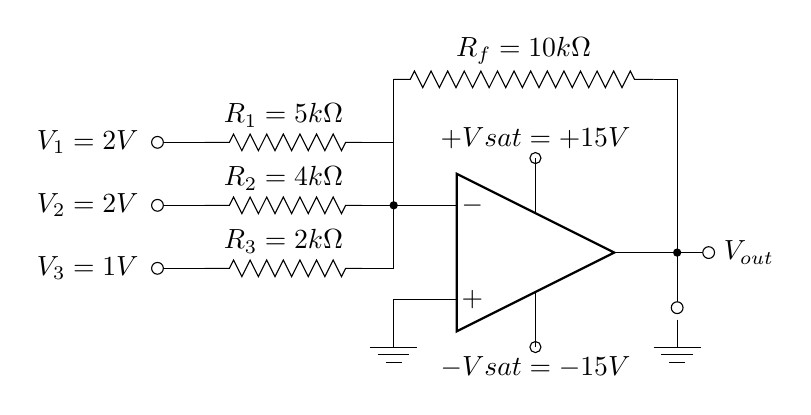
\begin{tikzpicture}[
    % Define custom styles using TikZ native features
    resistor/.style={
        circuitikz/resistor style/.style={},
        decorate, 
        decoration={zigzag, segment length=6pt, amplitude=3pt, pre length=6pt, post length=6pt}
    },
    terminal/.style={circle, draw, inner sep=1.5pt, fill=white},
    dot/.style={circle, fill, inner sep=1.2pt}
]

  % 1. Draw Op-Amp Triangle
  \draw[thick] (0,0) -- (0,2) -- (2,1) -- cycle;
  
  % Input Labels inside triangle (+ on bottom, - on top)
  \node at (0.2, 1.6) {$-$};
  \node at (0.2, 0.4) {$+$};

  % 2. Power Supply Lines
  \draw (1, 1.5) -- (1, 2.2) node[above] {$+\text{Vsat} = +15\text{ V}$};
  \draw (1, 2.2) circle (2pt);
  
  \draw (1, 0.5) -- (1, -0.2) node[below] {$-\text{Vsat} = -15\text{ V}$};
  \draw (1, -0.2) circle (2pt);

  % 3. Non-Inverting Input (+) Ground Connection
  \draw (0, 0.4) -- (-0.8, 0.4) -- (-0.8, -0.2);
  % Ground Symbol
  \draw (-1.1, -0.2) -- (-0.5, -0.2);
  \draw (-1.0, -0.3) -- (-0.6, -0.3);
  \draw (-0.9, -0.4) -- (-0.7, -0.4);

  % 4. Inverting Input (-) Node
  \draw (0, 1.6) -- (-0.8, 1.6) coordinate (invNode);
  \fill (-0.8, 1.6) circle (1.5pt);

  % 5. Three Input Resistors (R1, R2, R3)
  % R1 (Top)
  \draw (invNode) |- (-1.2, 2.4);
  \draw[resistor] (-1.2, 2.4) -- (-3.2, 2.4) node[midway, above=2pt] {$R_1 = 5\text{ k}\Omega$};
  \draw (-3.2, 2.4) -- (-3.8, 2.4) node[terminal] {} node[left] {$V_1 = 2\text{ V}\ $};

  % R2 (Middle)
  \draw (invNode) -- (-1.2, 1.6);
  \draw[resistor] (-1.2, 1.6) -- (-3.2, 1.6) node[midway, above=2pt] {$R_2 = 4\text{ k}\Omega$};
  \draw (-3.2, 1.6) -- (-3.8, 1.6) node[terminal] {} node[left] {$V_2 = 2\text{ V}\ $};

  % R3 (Bottom)
  \draw (invNode) |- (-1.2, 0.8);
  \draw[resistor] (-1.2, 0.8) -- (-3.2, 0.8) node[midway, above=2pt] {$R_3 = 2\text{ k}\Omega$};
  \draw (-3.2, 0.8) -- (-3.8, 0.8) node[terminal] {} node[left] {$V_3 = 1\text{ V}\ $};

  % 6. Feedback Resistor (Rf)
  \draw (invNode) -- (-0.8, 3.2);
  \draw[resistor] (-0.8, 3.2) -- (2.5, 3.2) node[midway, above=2pt] {$R_f = 10\text{ k}\Omega$};
  \draw (2.5, 3.2) -| (2.8, 1.0);

  % 7. Output Line and Terminal
  \draw (2, 1) -- (3.2, 1) node[terminal] {} node[right=2pt] {$V_{\text{out}}$};
  \fill (2.8, 1) circle (1.5pt);

  % Ground at Output Terminal
  \draw (2.8, 1) -- (2.8, 0.3) node[terminal] {};
  \draw (2.8, 0.15) -- (2.8, -0.2);
  % Ground Symbol
  \draw (2.5, -0.2) -- (3.1, -0.2);
  \draw (2.6, -0.3) -- (3.0, -0.3);
  \draw (2.7, -0.4) -- (2.9, -0.4);

\end{tikzpicture}
\end{center}

\begin{enumerate}
\item \text Derivation

Let the inverting input node (where $R_1,R_2,R_3,R_f$ meet) be node
$A$, and let the non-inverting input be grounded.

\text{Ideal op-amp assumptions:}

\begin{itemize}
\item\text{No current flows into either input terminal.}
\item\text{The open-loop gain is infinite, so the two inputs are forced to the same} \text{potential (virtual short).}
\end{itemize}

Since the non-inverting input is at $0\,\text{V}$ (grounded), the
virtual short forces node $A$ to also be at $0\,\text{V}$:

\begin{align}
V_A=0
\qquad(\text{virtual ground}).
\end{align}

Applying Kirchhoff's Current Law (KCL) at node $A$, the sum of
currents flowing into the node through $R_1,R_2,R_3$ must equal the
current flowing out through the feedback resistor $R_f$ (since no
current enters the op-amp input):

\begin{align}
\frac{V_1-V_A}{R_1}+\frac{V_2-V_A}{R_2}+\frac{V_3-V_A}{R_3}
=\frac{V_A-V_{\text{out}}}{R_f}.
\end{align}

Substituting $V_A=0$:

\begin{align}
\frac{V_1}{R_1}+\frac{V_2}{R_2}+\frac{V_3}{R_3}
=\frac{-V_{\text{out}}}{R_f}.
\end{align}

Solving for $V_{\text{out}}$:

\begin{align}
V_{\text{out}}
&=-R_f\left(\frac{V_1}{R_1}+\frac{V_2}{R_2}+\frac{V_3}{R_3}\right)\\
&=-\left(\frac{R_f}{R_1}V_1+\frac{R_f}{R_2}V_2+\frac{R_f}{R_3}V_3\right),
\end{align}


\begin{align}
V_{\text{out}}=-\sum_{i}\frac{R_f}{R_i}V_i.
\end{align}
\end{enumerate}

\begin{align}
V_{\text{out}}=-\left(\frac{R_f}{R_1}V_1+\frac{R_f}{R_2}V_2+\frac{R_f}{R_3}V_3+\cdots\right), \label{amplifier}
\end{align}

valid provided $V_{\text{out}}$ stays within the saturation limits,

\begin{align}
-V_{\text{sat}}\le V_{\text{out}}\le +V_{\text{sat}}.
\end{align}

% =========================================================
\item Wien Bridge Oscillator Frequency

For a Wien bridge oscillator with equal frequency-selective resistors
$R$ and capacitors $C$, the oscillation frequency is

\begin{align}
f_0=\frac{1}{2\pi RC}. \label{wien}
\end{align}

% =========================================================
\item Series RLC Circuit --- Resonance \label{resonance}

Kirchhoff's Voltage Law for a series $RLC$ circuit driven by
\begin{align}
v(t)=V_m\cos(\omega t)
\end{align}

\begin{align}
R\,i(t)+L\frac{di(t)}{dt}+\frac{1}{C}\int i(t)\,dt=v(t).
\end{align}

In the phasor domain, the impedance is

\begin{align}
Z(\omega)&=R+j\left(\omega L-\frac{1}{\omega C}\right)\\
|Z(\omega)|&=\sqrt{R^{2}+\left(\omega L-\frac{1}{\omega C}\right)^{2}}.
\end{align}

Converting to complex phasor notation 

\begin{align}
V(t) &= V_{\text{rms}} \sqrt{2} e^{j\omega t}\\
I(t) &= I_{\text{rms}} \sqrt{2} e^{j(\omega t - \phi)}
\end{align}
\begin{align}
Z(\omega) &= \frac{V(\omega)}{I(\omega)}\\
&= R + j\omega L + \frac{1}{j\omega C} \\
&= R + j\left(\omega L - \frac{1}{\omega C}\right)
\end{align}

Resonance occurs when the reactive part vanishes:

\begin{align}
\omega_0 L&=\frac{1}{\omega_0 C}\\
\implies \omega_0 &=\frac{1}{\sqrt{LC}}\\
f_0 &=\frac{\omega_0}{2\pi}.
\end{align}

At resonance, $Z(\omega_0)=R$, so

\begin{align}
I_{\text{rms}}(\omega_0)=\frac{V_{\text{rms}}}{R}. \label{res}
\end{align}

% =========================================================
\item Newton--Raphson Method

For a root of $f(x)=0$, the iterative update starting from $x_n$ is

\begin{align}
x_{n+1}=x_n-\frac{f(x_n)}{f'(x_n)}. \label{raphson}
\end{align}

% =========================================================
\item Logarithmic Decay Model

For a quantity that decays logarithmically with time,

\begin{align}
\sigma(t)=\sigma_0-k\ln(t),\qquad t\ge 1,
\end{align}

the difference between two times $t_1,t_2$ eliminates the unknown
constant $\sigma_0$:

\begin{align}
\sigma(t_2)-\sigma(t_1)&=-k\left[\ln(t_2)-\ln(t_1)\right]\\
&=-k\ln\!\left(\frac{t_2}{t_1}\right). \label{decay}
\end{align}


% =========================================================
\item [Gaussian (Normal) Function]
$X\sim\mathcal{N}(\mu,\sigma^{2})$, if 
\begin{align} 
	\label{eq:EE26BTECH11221-gaussian}
p_X(x)=\frac{1}{\sigma\sqrt{2\pi}}\,
\exp\!\left(-\frac{(x-\mu)^{2}}{2\sigma^{2}}\right),
\qquad -\infty<x<\infty.
\end{align}
%The \text{standard normal} form, with $\mu=0,\ \sigma=1$, is
%\begin{align}
%\phi(z)=\frac{1}{\sqrt{2\pi}}\,e^{-z^{2}/2},
%\qquad z=\frac{x-\mu}{\sigma}.
%\end{align}

The function is symmetric about $x=\mu$, and satisfies

\begin{align}
\int_{-\infty}^{\infty}f(x)\,dx=1,
\qquad
E[X]=\mu,
\qquad
\operatorname{Var}(X)=\sigma^{2}.
\end{align}


\begin{enumerate}

    \item Binomial Approximation (De Moivre--Laplace Theorem)
    For a binomial random variable $X \sim \text{Bin}(n, p)$ with large $n$ such that $np \ge 5$ and $n(1-p) \ge 5$, the binomial distribution can be approximated by a Gaussian distribution with:
    \begin{align}
    \mu = np, \quad \sigma^2 = np(1-p).
    \end{align}
    
    The probability mass function is approximated as:
    \begin{align}
    \pr{X = k} \approx \frac{1}{\sqrt{2\pi np(1-p)}} \exp\left( -\frac{(k - np)^2}{2np(1-p)} \right).
    \end{align}

    \item Continuity Correction
    When approximating a discrete binomial distribution using a continuous Gaussian distribution, a continuity correction factor of $0.5$ is applied:
    \begin{align}
    \pr{a \le X \le b} \approx P\left( \frac{a - 0.5 - np}{\sqrt{np(1-p)}} \le Z \le \frac{b + 0.5 - np}{\sqrt{np(1-p)}} \right).
    \end{align}

\end{enumerate}

% =========================================================
\item Central Limit Theorem (CLT)

Let $X_1,X_2,\dots,X_n$ be independent and identically distributed
(i.i.d.) random variables, each with finite mean $\mu$ and finite
variance $\sigma^{2}$ (the underlying distribution need not itself be
Gaussian). Define the sample mean

\begin{align}
\bar{X}_n=\frac{1}{n}\sum_{i=1}^{n}X_i.
\end{align}

Then, as $n\to\infty$, the standardized sample mean converges in
distribution to a standard normal random variable:

\begin{align}
Z_n=\frac{\bar{X}_n-\mu}{\sigma/\sqrt{n}}
\;\xrightarrow{d}\;
\mathcal{N}(0,1).
\end{align}

Equivalently, for large $n$,

\begin{align}
\bar{X}_n\ \approx\ \mathcal{N}\!\left(\mu,\ \frac{\sigma^{2}}{n}\right),
\qquad
\sum_{i=1}^{n}X_i\ \approx\ \mathcal{N}\!\left(n\mu,\ n\sigma^{2}\right).
\end{align}


% =========================================================
\item Effect of Scalar Multiplication on a Determinant

For an $n\times n$ matrix $A$ and scalar $k$,

\begin{align}
\det(kA)=k^{n}\det(A). \label{det}
\end{align}
% =========================================================
\item Notch (Band-Stop) Filter Response
\begin{align}
	\abs{H\brak{\j \omega}} = 
	\begin{cases}
0 & \omega = \omega_0, \\
\ne 0 & \text{otherwise} 
\end{cases}
\label{eq:EE26BTECH11221-notch}
\end{align}
% =========================================================
% QUESTION 4
% =========================================================
\item Which one of the following represents the frequency
response of a notch filter?

\hfill  (BM 2025)
% =========================================================
% OPTIONS WITH GRAPHS
% =========================================================
\begin{multicols}{2}
\begin{enumerate}
\setlength{\itemsep}{0pt}
% ---------------------------------------------------------
% OPTION A
% ---------------------------------------------------------

\item
\begin{center}
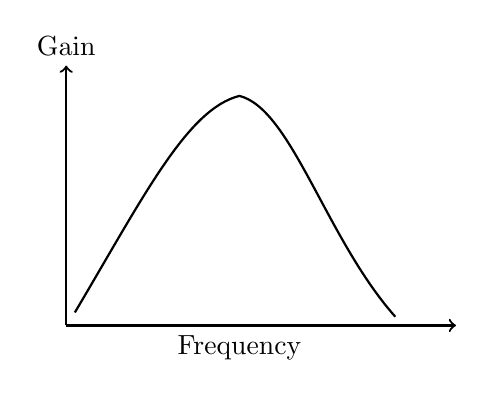
\begin{tikzpicture}[scale=1.1]

    % Axes
    \draw[->, thick] (0,0) -- (0,3);
    \draw[->, thick] (0,0) -- (4.5,0);

    % Labels
    \node[above] at (0,3) {Gain};
    \node[below] at (2,0) {Frequency};

    % Band-pass response
    \draw[thick]
        (0.1,0.15)
        .. controls (0.9,1.5) and (1.4,2.5) ..
        (2.0,2.65)
        .. controls (2.6,2.5) and (3.0,1.0) ..
        (3.8,0.1);

\end{tikzpicture}
\end{center}
% ---------------------------------------------------------
% OPTION B
% ---------------------------------------------------------
\item
\begin{center}
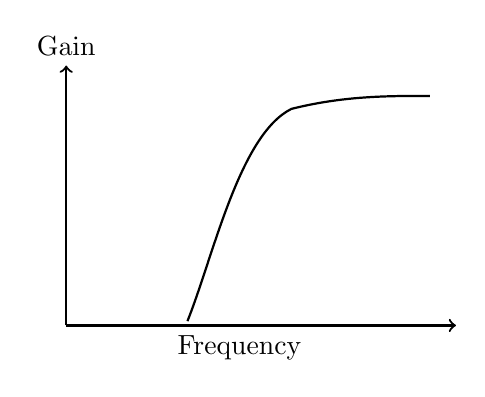
\begin{tikzpicture}[scale=1.1]

    % Axes
    \draw[->, thick] (0,0) -- (0,3);
    \draw[->, thick] (0,0) -- (4.5,0);

    % Labels
    \node[above] at (0,3) {Gain};
    \node[below] at (2,0) {Frequency};

    % High-pass response
    \draw[thick]
        (1.4,0.05)
        .. controls (1.7,0.8) and (2.0,2.2) ..
        (2.6,2.5)
        .. controls (3.2,2.65) and (3.7,2.65) ..
        (4.2,2.65);

\end{tikzpicture}
\end{center}

% ---------------------------------------------------------
% OPTION C
% ---------------------------------------------------------

\item
\begin{center}
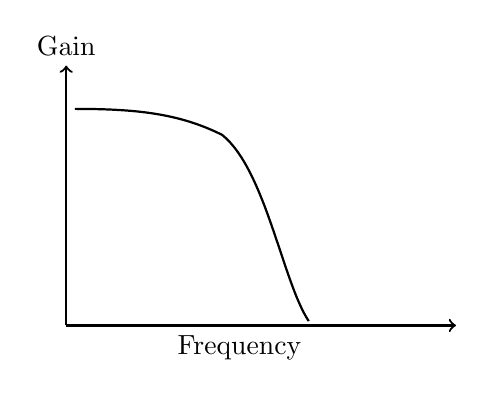
\begin{tikzpicture}[scale=1.1]

    % Axes
    \draw[->, thick] (0,0) -- (0,3);
    \draw[->, thick] (0,0) -- (4.5,0);

    % Labels
    \node[above] at (0,3) {Gain};
    \node[below] at (2,0) {Frequency};

    % Low-pass response
    \draw[thick]
        (0.1,2.5)
        .. controls (0.8,2.5) and (1.3,2.45) ..
        (1.8,2.2)
        .. controls (2.3,1.8) and (2.5,0.5) ..
        (2.8,0.05);

\end{tikzpicture}
\end{center}

% ---------------------------------------------------------
% OPTION D
% ---------------------------------------------------------

\item
\begin{center}
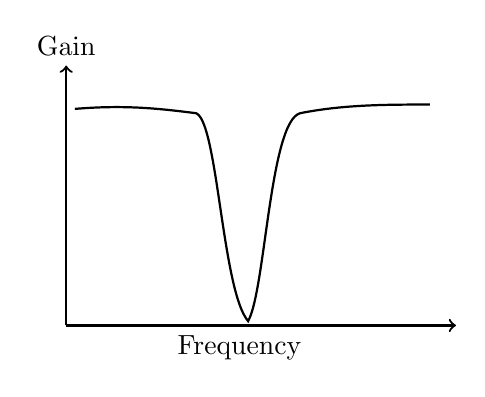
\begin{tikzpicture}[scale=1.1]

    % Axes
    \draw[->, thick] (0,0) -- (0,3);
    \draw[->, thick] (0,0) -- (4.5,0);

    % Labels
    \node[above] at (0,3) {Gain};
    \node[below] at (2,0) {Frequency};

    % Notch response
    \draw[thick]
        (0.1,2.5)
        .. controls (0.7,2.55) and (1.1,2.5) ..
        (1.5,2.45)
        .. controls (1.75,2.35) and (1.8,0.4) ..
        (2.1,0.05)
        .. controls (2.3,0.4) and (2.35,2.35) ..
        (2.7,2.45)
        .. controls (3.2,2.55) and (3.7,2.55) ..
        (4.2,2.55);

\end{tikzpicture}
\end{center}
\end{enumerate}
\end{multicols}
% =========================================================
% SOLUTION
% =========================================================
\solution
From \eqref{eq:EE26BTECH11221-notch},
d). 
\end{enumerate}
%\end{document}
